% Chapter Template

\chapter{Pre-Processing and Post-Processing Scheme for Fluorescence Microscopy Images} % Main chapter title

\label{chap:Chapter4} % Change X to a consecutive number; for referencing this chapter elsewhere, use \ref{ChapterX}

%\textcolor{red}{There are many factors that degrade the quality of images. The knock-on effect is sub-optimal segmentation results. List the problems and show some images of them. What techniques exist to curb these negative effects? Although it is very common for preprocessing to be done before any further analysis, lack of a scheme. Where do we take this up from (after PSF deconvolution). Why is it non-trivial to design criteria for an ideal image to segment? What do we plan to accomplish in this section?}

Fluorescence microscopy has become an indispensable tool \citep{Matula2012} in myriad of scientific disciplines such as chemistry, biology, neurobiology and medicine to name a few. It gives scientists visual access to physiological processes and other cellular and sub-cellular activities.
Fluorescence microscopy coupled with the tremendous technological advancement of image acquisition has lead to an explosion of raw image data such that the sheer volume of images acquired presents too much of a burden on manual analysis \citep{Matula2012}.
Consequently, there is a need for highly accurate automated analysis.
In such image analysis, image segmentation has established itself as a key process in identifying and extracting objects of interest which can thereafter be used in higher level image analysis.
The ever increasing demand on image segmentation is to extract the objects of interest with greater accuracy in a shorter time.

There are many factors that degrade the quality of fluorescence images and these can result in sub-optimal segmentations.
%affect the accuracy of the segmentation.
These factors have been studied independently to a great deal and have been successfully applied to real-world data.
Some of these problems are poor contrast, photo-bleaching, a not black enough blackground, non-fluorescence of samples, improper excitation, etc.

Literature is rich with techniques that are able to, a high degree, negate the effect of these factors \cite{Lysaker2004,Wang2008,Zhou2013}. There is, however, a lack of definition of a scheme prior to segmentation that prepares an image such that accurate segmentation can be achieved.

The task of defining a set of criteria an image has to meet for reliable segmentation results is not a trivial one. However, there are some basic notions that an image can be tuned towards which would present a better image for the purpose of segmentation.
%obtained,
Image enhancement on the original image can be done to facilitate higher level analysis e.g. contrast enhancement.
%segmentation qualities. The criteria of this scheme is
This paper aims to design a hybrid algorithm that builds on highly successful algorithms to produce better results. The process emphasises
\begin{enumerate}
	\item Noise reduction
	\item Object data enhancement
	\item Edge completion and enhancement
	\item Reduction of intra-region variance
\end{enumerate}

\begin{figure}[!h]
	\centering
	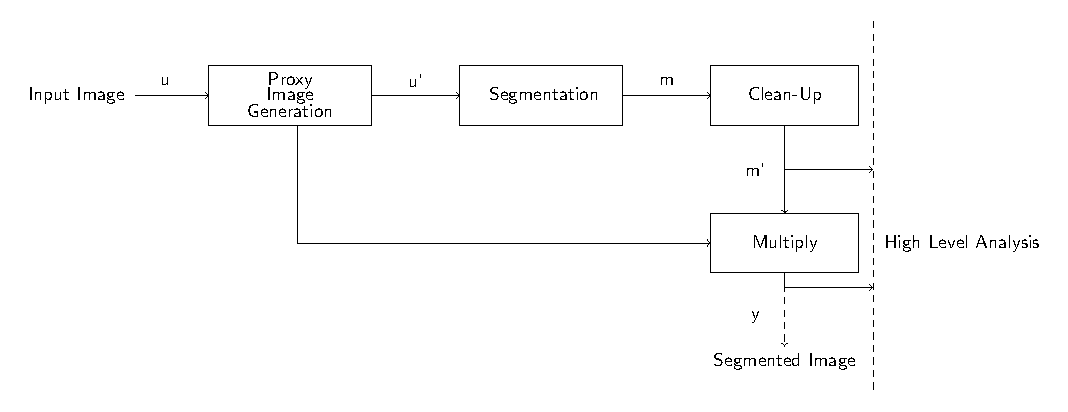
\includegraphics[width=1\columnwidth]{mypreprocess/whole_process}
	\caption{Segmentation Scheme.}
	\label{fig:wholescheme}
\end{figure}

\begin{figure}[!h]
	\centering
	%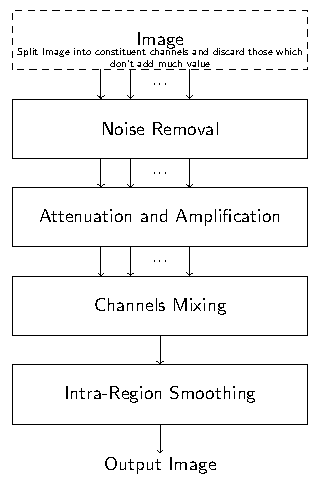
\includegraphics[width=0.25\columnwidth]{mypreprocess/proposed_scheme}
	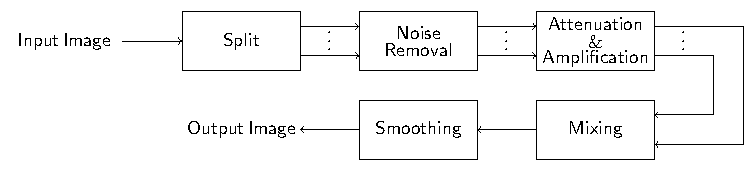
\includegraphics[width=1\columnwidth]{mypreprocess/preprocess_flow}
	\caption{Proxy image generation.}
	\label{fig:flowchartproposedscheme}
\end{figure}

%----------------------------------------------------------------------------------------
%	SECTION 1
%----------------------------------------------------------------------------------------

%\section{Fluorescence Image Properties}
%\label{sec:imageproperties}
%
%\textcolor{red}{Make a relation to it's impact on segmentation quality. 
%	Noise: type and mathematical model. 
%	Extreme low contrast issues.
%	Edge enhancement and completion}

%----------------------------------------------------------------------------------------
%	SECTION 2
%----------------------------------------------------------------------------------------

\section{Preprocessing Scheme}
\label{sec:preprocessscheme}


%----------------------------------------------------------------------------------------
%	SUBSECTION 1
%----------------------------------------------------------------------------------------

\subsection{Denoising}
\label{sec:PoissonDenoising}

\begin{definition}[Removing useless channels]
	Many segmentation algorithms are designed to work on gray scale images. If we have a colour image it is first converted to gray scale. Through the advancements in optical engineering it is now possible for fluorescence images to be obtained in colour, however not all channels add object data to the image. They in fact degrade the image due to the noise in that channel.  Often enough, these redundant channels will just be "data-less and noisy", so eliminating this channel will provide a huge improvement for segmentation purposes.
	%A direct conversion of the colour image to a gray scale image yields poor results as seen in Figure \ref{fig:test_gray}. In Figure \ref{fig:test_orig}, there is clearly no blue-channel data in the image, as a result when the image is converted to gray scale, as shown in Figure \ref{fig:test_gray}, the red-channel data is significantly suppressed due to the averaging of the channels that occurs when the conversion to gray scale takes place. In this case, the redundant blue-channel can be discarded entirely which yields Fig. \ref{fig:test_chanmixgray}.
\end{definition}

\begin{definition}[Poisson Noise Reduction]
	In \Cref{sec:PoissonDenoising} and \Cref{sec:ImageProcessing} we mentioned that the primary form of noise in fluorescent images is Poisson noise. It is important to remove as much noise as possible without dampening the boundary information. To this end we've used the Total-Variation anisotropic denoising (Bregman Split). Although it was developed to remove Gaussian noise, it was shown by Rodriguez \textit{et al.}\citep{Rodriguez2008} that is supersedes other state-of-the-art Poisson noise removal methods, e.g.  wavelets \citep{Timmermann1999}, platelets\citep{Willett2004}, minimum description length \citep{Nowak1999}, while maintaining signal integrity. 
	
	The Poisson distribution, which has equal mean and standard deviation i.e. $\mu = \sigma$, is defined by
	\begin{equation}
	P(n,\mu) = \frac{e^{-\mu}\mu^{n}}{n!}
	\label{eq:poissondist}
	\end{equation}
	
	Let $y = \lbrace y_i:i=1, \cdots, N \rbrace$ and $x = \lbrace x_i:i=1, \cdots, N \rbrace$ be the observed and the true image, respectively. The sample $y_i$ is a Poisson contaminated form of $x_i$. We desire to recover the signal $x$ from the observed signal $y$. From Bayes' Law we get
	\begin{equation}
	P(x \vert y) = \frac{P(y \vert x)P(x)}{P(y)}
	\label{eq:bayeslaw}
	\end{equation}
	Therefore, we wish to find the maximum of $P(y \vert x)P(x)$. If all samples are affected by Poisson noise we have
	\begin{equation}
	P(y \vert x) = P(y,x) = \frac{e^{-x_i}x_i^{y_i}}{y_i!}
	\label{eq:poissonafect}
	\end{equation}
	Thus the likelihood of observing $y$ given the true image $x$ is given by
	\begin{equation}
	P(y \vert x) = \prod_{i=1}^{N} \frac{e^{-x_i}x_i^{y_i}}{y_i!}
	\label{eq:poissonlikelihood}
	\end{equation}
	
	
	In anisotropic TV denoising we wish to recover the original image given the noisy image by minimising the constrained problem
	
	\begin{equation}
	\underset{u} {\mathrm{min}} \left| \left| \frac{du}{dx} \right| \right|_1 + \left| \left| \frac{du}{dy} \right| \right|_1 + \frac{\mu}{2} \left| \left| u-f \right| \right|^2_2
	\label{equ:anisotropic_tv_constrained}
	\end{equation}
	where $\mu > 0$ is the regularisation parameter which affects the balance between noise removal and signal preservation \citep{Getreuer2012}, $u$ is the true image and $f$ is the noisy image. We actually solve the unconstrained problem
	\begin{equation}
	\underset{u, dx, dy} {\mathrm{min}} \left| \left|dx_1 \right| \right|_1 + \left| \left| dy_1 \right| \right|_1 + \frac{\mu}{2} \left| \left| u-f \right| \right|^2_2 +
	\frac{\lambda}{2} \left| \left| dx-u_x \right| \right|^2_2 + \frac{\lambda}{2} \left| \left| dy-u_y \right| \right|^2_2
	\label{equ:anisotropic_tv_unconstrained}
	\end{equation}
	This can be solved using the Bregman Split algorithm \citep{Wei2010}.
	The algorithm is run iteratively until the error, $e = \frac{\vert u'-u \vert}{\vert u \vert}$ where $u'$ is the image obtained after denoising the input image $u$, is less than a user-defined tolerance factor, $\epsilon$. 
	%We used  $\mu=20$, $\lambda=1$ and $\epsilon=1 \times 10^{-3}$, the original and the denoised channels are shown in Figures \ref{fig:gchannel_1_orig}, \ref{fig:rchannel_1_orig}, \ref{fig:gchannel_1_denoised} and \ref{fig:rchannel_1_denoised}
\end{definition}
%----------------------------------------------------------------------------------------
%	SUBSECTION 2
%----------------------------------------------------------------------------------------

\subsection{Separation under Intensity}
\label{sec:contrastcorrection}

The fundamental principle underlying binary image segmentation is to split-up an image into regions, where regions that are labelled $l_0$ share similar values with with regard to the feature under consideration. This also means that there is high dissimilarity with the regions that are labelled $l_1$. For grayscale images, such as the type we are concerned with, this feature is generally intensity. With respect to segmentation with regard a feature, an ideal image is one where there isn't an overlap in the feature space between the background and the object, as illustrated in \Cref{fig:featuredataset}. In real images (non-synthetic) this is almost never the case as there is no known feature space or it does not exist.

\begin{figure}[!h]
	\centering
	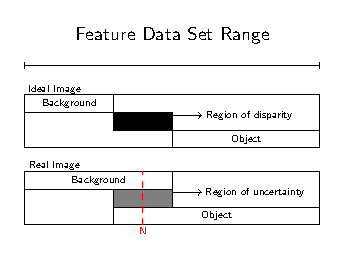
\includegraphics[width=0.5\columnwidth]{feature_data_set}
	\caption{Feature data set.}
	\label{fig:featuredataset}
\end{figure}

Grayscale medical image segmentation typically uses intensity as the dominant feature on which the applied segmentation algorithms are biased. Hence, it is common to precede segmentation by contrast enhancement \citep{Kim2003,Subr2005}. The problem here lies with the fact that the aim contrast enhancement is to bring out the details more clearly that are otherwise obscured due to limited dynamic range, non-uniform illumination, etc. In fluorescence image this does not necessarily mean that the enhanced image posesses better segmentation qualities, in terms of intensity.

In this section we present a novel mapping function whose aim is to shrink the "region of uncertainty" by non-linearly widening the gap between background pixels and object pixels. This function is composed of two piecewise sub-functions; one for data attenuation and one for data amplification. We first design the properties the mapping function should have. 

\begin{definition}[Remapping Function Properties]
	The remap function is denoted as $\widetilde{x_i} = R(x_i)$, where $\widetilde{x_i}$ is the new value which remaps the input pixel, $x_i$, using the function $R$. The range on which $R$ works is $[0,L]$, where $0$ and $L$ represent the lowest and highest values a pixel can take respectively. For 8-bit gray scale images the highest value is usually $L=255$. Let the value that represents the greatest classification uncertainty be denoted $N$, as illustrated in \Cref{fig:featuredataset}.
\end{definition}

\begin{enumerate}
	\item{}
	\textit{$R$ must be non-decreasing in the interval $[0, L]$}\\
	This is a trivial criterion arising from the context in which our problem is defined. We are speciffically focussing on non-inverted fluorescence images therefore the background  will ideally be black. Consequently, it is not possible for a lower intensity pixel to have a higher probability of belonging to the object compared to a pixel of a higher gray level intensity. 
	
	\item
	\textit{$\widetilde{x_i} = R(x_i=N) = N$}\\
	This value has no bias as to whether it tends more to the background or the object. It is best left unaltered.
	
	\item
	\textit{Attenuation: $\widetilde{x_i} < x_i, \, \forall x_i<N$}\\
	$R$ must remap gray-level intensities below $N$, according to $0 \leq \widetilde{x_i} \leq x_i$.
	
	\item
	\textit{Amplification: $\widetilde{x_i} > x_i, \, \forall x_i>N$}\\
	$R$ must remap gray-level intensities above $N$, according to $x_i \leq \widetilde{x_i} \leq L$.
	
	\item
	\textit{$R'$ must be non-decreasing in the interval $[0,N]$}\\
	Given two pixels, $p_1$ and $p_2$, with values $x_1$ and $x_2$ respectively where $x_1<x_2$. It is more probable for $p_2$ to belong to the object since it has a higher value. Also, pixels with gray levels intensities closer $0$ do not need to be attenuated as much.
	
	\item
	\textit{$R'$ must be non-increasing in the interval $[N,L]$}\\
	As the pixels values approach $L$, less amplification is needed since the pixels are already more likely to be classified as belonging to the object.
\end{enumerate}

\begin{definition}[Function Design]
	Many functions can be designed given the criteria presented. We have decided that one of the better solutions is to make the mapping function a piece-wise quadratic Bezier curve. The motivation for this is its appeal in easy and intuitive tuning of the sub-functions. The two functions are $R_{att}$, for the attenuation section, and $R_{amp}$, for the amplification section as shown in \Cref{fig:remapfcn}.
	
	There are three anchor pointsthe function must pass through. These are $p_0(0,0)$, $p_2(N, N)$ and $p_4(L,L)$. If the curve between $p_0$ and $p_2$ is a straight line and if the curve between $p_2$ and $p_4$ is a straight line then there is no change between the output and input image since the gradient of the line segments are equal and equal to $1$. Additional control points are needed to bend the curve.
	There is a particular class of curves whose shapes are useful for our purpose. This places constraints on the position of the control points. Relative to the straight line, $y=x, \, x \in [0,L]$, the amplification curve would be above the relaxed line, $p_{3y} > p_{3x}$, and similarly the attenuation curve would be below the line, $p_{1y} < p_{1x}$. Also, given that the function is to be a one-to-one function, the control point for the attenuation function $p_{1x}<N$; similarly the control point for the amplification function $p_{3x}>N$.
	
	\begin{figure}[!h]
		\centering
		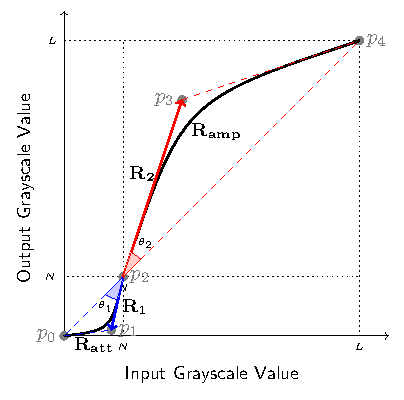
\includegraphics[width=0.60\columnwidth]{remapfcn.pdf}
		\caption{Plot of remapping function.}
		\label{fig:remapfcn}
	\end{figure}
	
	The controls points in the Cartesian representation don't say much about the amount of tension in the curve. A more useful representation is to represent the control point implicitly as an angular deviation of the straight line and a magnitude, $p_c(R_c, \theta_c)$. Where $\theta_c \in [0, \frac{\pi}{4}]$ and $R_c \in \mathbb{R}^+$. The angular deviation is the measure off the straight line which is counter-clockwise for the amplification function and clockwise for the attenuation function. The deviation, $\theta_c$, where $c \in {1,2}$, away from the straight line is further implicitly represented as a range $\kappa_c \in [0,1]$ where $\kappa_c=0$ implies $\theta_c = 0$ would mean no deviation, and $\kappa_c = 1$ implies $\theta_c = \frac{\pi}{4}$ would mean maximum deviation.
	The only real advantage in defining the function this way is that the parameters are more geometrically correlated to the curve. As the curve approaches the ends of it domain, less attenuation/amplification occurs, which meets criterions 5 and 6.
	
	\begin{figure}[!t]
		\centering
		\subfigure[Amplification function controls points.]
		{
			
			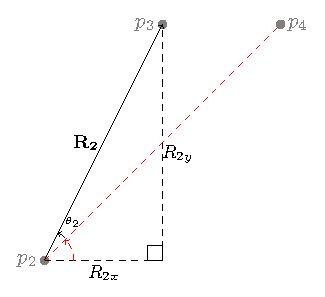
\includegraphics[width=0.48\columnwidth]{attenutation_control_points.pdf}
			\label{fig:ampcontrolpoints}
		}	
		\subfigure[Amplification function curve.]
		{
			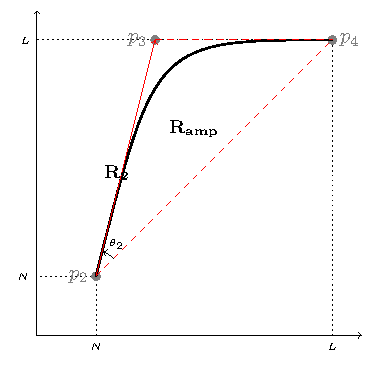
\includegraphics[width=0.48\columnwidth]{attenutation_curve.pdf}
			\label{fig:ampcurve}
		}
		\caption{Amplification function control points and curve.}
		\label{fig:ampcalculation}
	\end{figure}

	The position of the attenuation control point is calculated as
	\begin{equation*}
		{p_1} = \left(
		p_{2x} - R_1\cos[\frac{\pi}{4}(1+\kappa_1)],
		p_{2y} - R_1\sin[\frac{\pi}{4}(1+\kappa_1)]
		\right)
	\end{equation*}
	Similarly, the position of the amplification control point, as shown in \Cref{fig:ampcalculation}, can be calculated as
	\begin{equation*}
		{p_3} = \left(
		p_{2x} + R_2\cos[\frac{\pi}{4}(1+\kappa_2)],
		p_{2y} + R_2\sin[\frac{\pi}{4}(1+\kappa_2)]
		\right)
	\end{equation*}
	
	The piecewise functions that define the curve are given by	
	\begin{eqnarray}
		R_{att}(t) = \sum_{i=0}^2 p_i J_i^n \\
		R_{amp}(t) = \sum_{i=2}^4 p_i J_i^n
	\end{eqnarray}
	Where $J_i^n$ is the Bernstein basis function, defined as
	\begin{equation}
	J_i^n = \begin{pmatrix}
	n \\
	i
	\end{pmatrix}	
	t^i(1-t)^{n-i}, \,\, t \in [0,1]
	\label{eq:bernsteinbasis}
	\end{equation}
	
	For each input gray level intensity $x \in [0, L]$ we require corresponding output gray level intensity $y \in [0, L]$.
	The curve is expressed as a parametrisation with respect to $t$ for each of its $x$ and $y$ parameters.
	For a curve defined by three control points $q_0$, $q_1$ and $q_2$ where $q_0 < q_1 < q_2$, the equation for the curve determine by these points is the quadratic bezier given by
	\begin{equation}
		R = \sum_{i=0}^2 q_i J_i^n
	\end{equation}
	
	For a quadratic bezier curve, this simplifies to
	\begin{align*}
		R &= q_0(1-t)^2 + 2q_1(1-t)t + q_2t^2 \\
		0 &= (q_0-2q_1+q_2)t^2 + (-2q_0+2q_1)t + (q_0-R)
	\end{align*}
	
	Therefore for the parametric function $R_x$, we require the set of values of $t$ for which $R_x \in [q_{0x},q_{2x}]$. The value of $t$ for a given $R_x$ is determined by the solution to the quadratic equation.\\
	Let $a=q_{0x}-2q_{1x}+q_{2x}$, $b=-2q_{0x}+2q_{1x}$, and $c=q_{0x}-R_x$.\\
	It is seen that $b>0$, since $q_{1x} > q_{0x}$, and $c \leq 0$, since $R_x \geq q_{0x}$.\\
	Rewrite $a$ as $a=(q_{0x}-q_{1x}) + (q_{2x}-q_{1x})$.
	For the case of $a$, there are two cases.
	
	\begin{enumerate}
		\item
		For $q_{1x} \in [q_{0x}, \frac{q_{2x}-q_{0x}}{2}]$, $a>0$.\\
		In this case $-4ac>0$ hence $\sqrt{b^2-4ac}>b$.\\
		$\therefore$ the only value of $t$ which is positive and must be the solution is given by
		\begin{equation}\label{eq:qt1}
			t =  \frac{(q_{1x}-q_{0x}) + \sqrt{R_x(q_{0x}-2q_{1x}+q_{2x})+(q_{1x}^2-q_{0x}q_{2x}})}{q_{0x}-2q_{1x}+q_{2x}}
		\end{equation}

		\item
		For $q_{1x}>\frac{q_{2x}-q_{0x}}{2}$, $a<0$.\\
		It is known that a real solution exists. This means that
		\begin{align*}
			b^2 -4ac &\geq 0 \\
			b^2 &\geq 4ac \\
			\implies \sqrt{b^2-4ac} &< b
		\end{align*}
		$\therefore$ the only value of $t$ which is positive and must be the solution is given by
		\begin{equation}\label{eq:qt2}
			t =  \frac{(q_{1x}-q_{0x}) + \sqrt{R_x(q_{0x}-2q_{1x}+q_{2x})+(q_{1x}^2-q_{0x}q_{2x}})}{q_{0x}-2q_{1x}+q_{2x}}
		\end{equation}
	\end{enumerate}

	In both cases the solution to $t$ can be calculated using the same formula.
	It is possible for the remapping function to exceed the range, in this case any value that maps to a value higher than the maximum value will be assigned the maximum value i.e. $\widetilde{x_i} = min(R(x_i),L), \,  x_i \in (N,L]$; similarly any value that maps to a value lower than the minimum value will be assigned the minimum value i.e. $\widetilde{x_i} = max(R(x_i),0), \, x_i \in [0,N)$.
\end{definition}

\begin{definition}[Function Properties and Constraints]
This function presents several properties within the constraints defined a follows:
\begin{enumerate}
	\item
	The curves obey the convex hull property. The sub-functions will always be contained within the control polygon determined by the control points \citep{Vince2006,Marsh2005}.
	
	\item
	No attenuation when $\kappa_1=0$ and no amplification when $\kappa_2=0$.
	
	\item
	$R$ is continuous in $x_i \in [0,L]$.
	
	\item
	$R$, is weakly monotonically increasing in $x_i \in [0,L]$.
	
	\item
	$R'_{att}$, is monotonically increasing in $x \in [0, N]$.
	
	\item
	$R'_{amp}$, is monotonically decreasing in $x \in [N, L]$.
	
	\item
	The ends of the curve are coincident with the first and last control points of the control polygon.
	
	\item
	The direction of the tangent vectors from the end points of the curve are the same as the direction of the vector anchored at the control point and along the line that joins the end point and the centre control point of the control polygon \citep{Vince2006,Marsh2005}.
\end{enumerate}
\end{definition}


%----------------------------------------------------------------------------------------
%	SUBSECTION 3
%----------------------------------------------------------------------------------------

\subsection{Channel Mixing}
\label{sec:channelmixing}

To reconstitute an image from the updated channels we perform channel mixing. In an eqi-weighted mixing system, each channel contributes equally to the mixed-down image. This simplistic method of channel mixing does not always produce the best image.
A consequence, of equi-weighted mixing is that some channels might become very suppressed and may be disregarded by the segmentation algorithm. Hence, it is necessary to assign weights which are channel dependant. These weightings must sum to one, $\sum_{i \in C} w_i = 1$, where $C$ is the set of channels to be mixed-down. The mixed-down image is then calculated as $y = \sum_{i \in C}w_iC_i$, where $C_i$ is channel $i$. Channels with very low gray level values are given a greater weight.

%We used $w_R=0.5$, $w_G=0.5$, and $w_B=0.0$ to produce Figure \ref{fig:mixingchannels}, where $w_X$ is the contribution of channel X to the mixed-down image. 


%----------------------------------------------------------------------------------------
%	SUBSECTION 4
%----------------------------------------------------------------------------------------

\subsection{Intra-Region Smoothing and Edge Completion and Enhancement}
\label{sec:Diffusion}

One of the criteria which is used in identifying an image is that objects tend to have little intra-region variance.
It is common for fluorescence images to be plagued with various degrees of lighting and contrast even within objects. This is primarily due to improper excitation, non-fluorescence of particles and ubiquitous measurement errors during acquisition.
In some cases it is easy to visualise the completed edge of the object by joining the disconnected edge components where the extension is along the direction of the edge.
We used a coherence enhancing diffusion filter with optimised rotational invariance (CED-ORI) presented in \citep{Weickert1999,Weickert2002,Weickert2003}, which very successfully reduces intra-region variance and joins closely-disconnected edges.

The diffusion works by evolving the image, $u$, over a time using $n$ discrete time steps, $t$, called the diffusion time. The evolution equation is defined as:
\begin{equation}
\frac{\partial u}{\partial t} = \nabla \cdot (D\nabla u)
\end{equation}
where $D = \begin{pmatrix}
a & b \\
b & c
\end{pmatrix}$ is the diffusion tensor which can be adapted to the local image structure measure known as the structure tensor. The structure tensor is given by:
\begin{equation}
J_{\rho}(\nabla u_{\sigma}) = G_{\rho} \ast (\nabla u_{\sigma} \nabla u_{\sigma}^T)
\end{equation}
Where $G_{\rho}$ is the Gaussian kernel with standard deviation $\rho$, and $u_{\sigma} := G_{\sigma} \ast u$ where $G_{\sigma}$ is the Gaussian kernel with standard deviation $\sigma$.
The eigenvalues of $J_{\rho}=\begin{pmatrix}
J_{11} & J_{12} \\
J_{12} & J_{22}
\end{pmatrix}$ are
\begin{eqnarray}
\mu_{1} = \frac{1}{2}\left( J_{11} + J_{12} + \sqrt{(J_{11}-J_{22})^2+4J_{12}^2} \right) \\
\mu_{2} = \frac{1}{2}\left( J_{11} + J_{12} - \sqrt{(J_{11}-J_{22})^2+4J_{12}^2} \right)
\end{eqnarray}
Where the normalised first eigenvector satisfies
\begin{equation}
\begin{pmatrix}
cos \alpha \\
sin \alpha
\end{pmatrix} \parallel
\begin{pmatrix}
2J_{12} \\
J_{22}-J_{11}+\sqrt{(J_{11}-J_{22})^2 + 4J_{12}^2}
\end{pmatrix}
\end{equation}
The diffusion tensor's, $D$, eigenvectors are obtained from the structure tensor eigenvectors using:
\begin{eqnarray}
\lambda_1 &=& c_1 \\
\lambda_2 &=& \left\lbrace \begin{matrix}
c_1 & \text{if } \mu_1=\mu_2 \\
c_1+(1-c_1)e^{\frac{c_2}{(\mu_1-\mu_2)^2}}& \text{otherwise}
\end{matrix}
\right.
\end{eqnarray}
where $c_1 \in (0,1)$, $c_2>0$. The elements of $D$ are then calculated as:
\begin{eqnarray}
a = \lambda_1 cos^2 \alpha + \lambda_2 sin^2 \alpha \\
b = (\lambda_1 - \lambda_2)sin \alpha cos \alpha \\
c = \lambda_1 sin^2 \alpha + \lambda_2 cos^2 \alpha
\end{eqnarray}
Further details on the coherence enhancing diffusion filter with optimised rotational invariance is found in \cite{Weickert2002}. In \citep{Maska2013} and \citep{Kroon2009} this filter was used primarily for noise removal while preserving edge detail, here we use it for its edge completion and smoothing properties.
%The comparison between the original image and the final image is shown in Figure  \ref{Org_dif}, the diffused image appears very distorted however the data necessary for the object extraction is present with less intra-region variance and better edge coherence. These added qualities are vital to yield optimal segmentations.

%----------------------------------------------------------------------------------------
%	SECTION 3
%----------------------------------------------------------------------------------------

\section{Experimental Results}
\label{sec:preprocessschemeexperimentalresults}

\begin{figure}[!h]
	\centering
	\subfigure[]
	{
		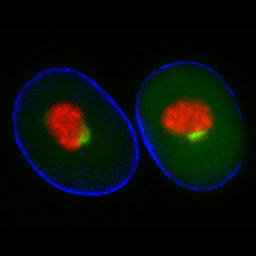
\includegraphics[width=0.23\columnwidth]{mypreprocess/1colr}
		\label{fig:1colr}
	}
	\subfigure[]
	{
		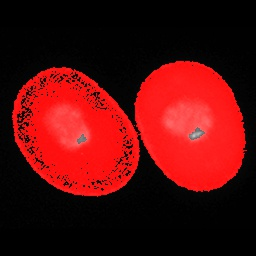
\includegraphics[width=0.23\columnwidth]{mypreprocess/1gray}
		\label{fig:1g}
	}
	\subfigure[]
	{
		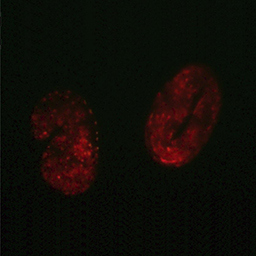
\includegraphics[width=0.23\columnwidth]{mypreprocess/3colr}
		\label{fig:3colr}
	}
	\subfigure[]
	{
		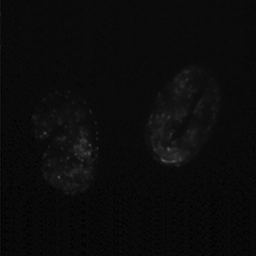
\includegraphics[width=0.23\columnwidth]{mypreprocess/3g}
		\label{fig:3g}
	}
	\subfigure[]
	{
		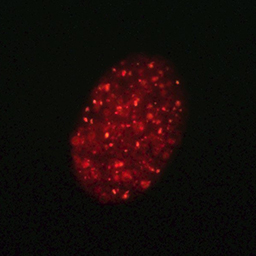
\includegraphics[width=0.23\columnwidth]{mypreprocess/4colr}
		\label{fig:4colr}
	}
	\subfigure[]
	{
		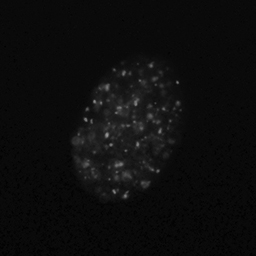
\includegraphics[width=0.23\columnwidth]{mypreprocess/4g}
		\label{fig:4g}
	}
	\subfigure[]
	{
		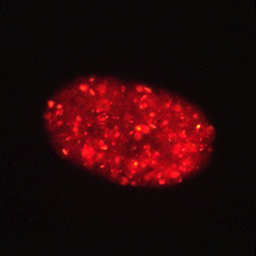
\includegraphics[width=0.23\columnwidth]{mypreprocess/5colr}
		\label{fig:5colr}
	}
	\subfigure[]
	{
		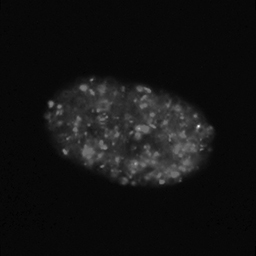
\includegraphics[width=0.23\columnwidth]{mypreprocess/5g}
		\label{fig:5g}
	}
	\caption{Original images with direct conversion to grayscale.}
	\label{fig:originaltogray}
\end{figure}

\begin{figure}[!t]
	\centering
	\subfigure[]
	{
		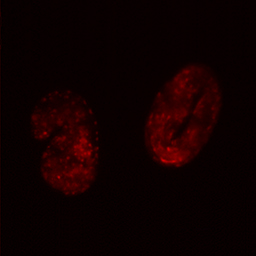
\includegraphics[width=0.23\columnwidth]{mypreprocess/3colr_removenoisychannels}
		\label{fig:3colnoiseless}
	}
	\subfigure[]
	{
		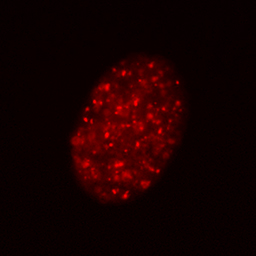
\includegraphics[width=0.23\columnwidth]{mypreprocess/4colr_removenoisychannels}
		\label{fig:4colnoiseless}
	}
	\subfigure[]
	{
		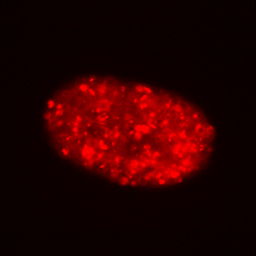
\includegraphics[width=0.23\columnwidth]{mypreprocess/5colr_removenoisychannels}
		\label{fig:5colnoiseless}
	}

	\subfigure[]
	{
		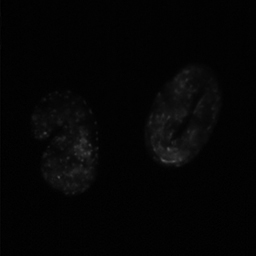
\includegraphics[width=0.23\columnwidth]{mypreprocess/3g_removenoisychannels}
		\label{fig:3gnoiseless}
	}
	\subfigure[]
	{
		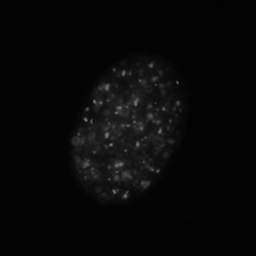
\includegraphics[width=0.23\columnwidth]{mypreprocess/4g_removenoisychannels}
		\label{fig:4gnoiseless}
	}
	\subfigure[]
	{
		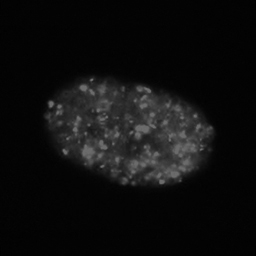
\includegraphics[width=0.23\columnwidth]{mypreprocess/5g_removenoisychannels}
		\label{fig:5gnoiseless}
	}
	\caption{Removed noisy channels with corresponding grayscale images.}
	\label{fig:noiselessimages}
\end{figure}

\begin{figure}[!h]
	\centering
	\subfigure
	{
		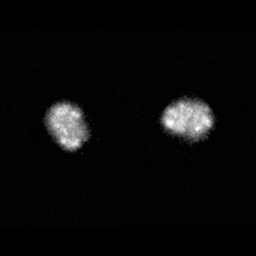
\includegraphics[width=0.23\columnwidth]{mypreprocess/1r.jpg}
		\label{fig:1r}
	}
	\subfigure
	{
		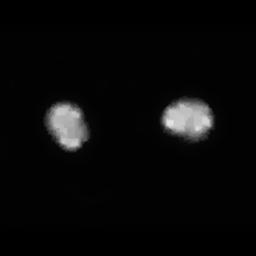
\includegraphics[width=0.23\columnwidth]{mypreprocess/1rtv.jpg}
		\label{fig:1rtv}
	}
	\subfigure
	{
		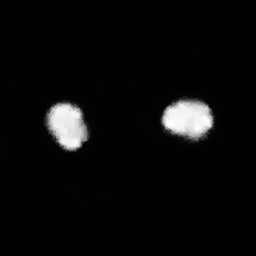
\includegraphics[width=0.23\columnwidth]{mypreprocess/1rtv_remapped.jpg}
		\label{fig:1rremap}
	}

	\subfigure
	{
		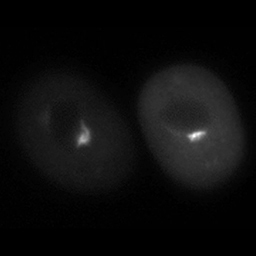
\includegraphics[width=0.23\columnwidth]{mypreprocess/1g.jpg}
		\label{fig:1gg}
	}
	\subfigure
	{
		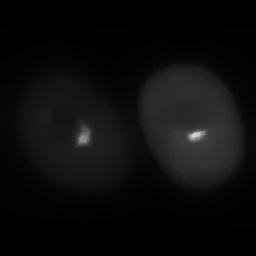
\includegraphics[width=0.23\columnwidth]{mypreprocess/1gtv.jpg}
		\label{fig:1gtv}
	}
	\subfigure
	{
		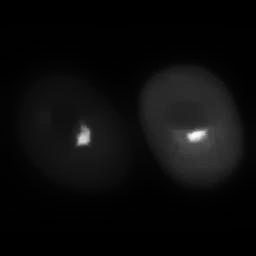
\includegraphics[width=0.23\columnwidth]{mypreprocess/1gtv_remapped.jpg}
		\label{fig:1gremap}
	}
	
	\subfigure
	{
		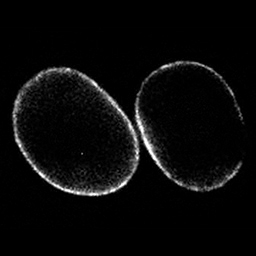
\includegraphics[width=0.23\columnwidth]{mypreprocess/1b.jpg}
		\label{fig:1b}
	}
	\subfigure
	{
		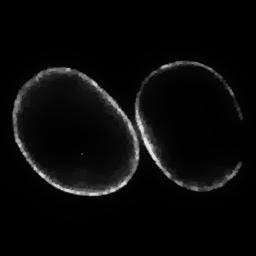
\includegraphics[width=0.23\columnwidth]{mypreprocess/1btv.jpg}
		\label{fig:1btv}
	}
	\subfigure
	{
		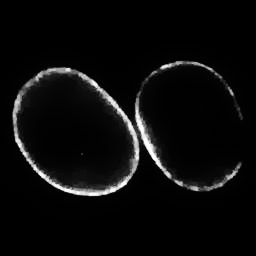
\includegraphics[width=0.23\columnwidth]{mypreprocess/1btv_remapped.jpg}
		\label{fig:1bremap}
	}
	
	\subfigure	
	{
		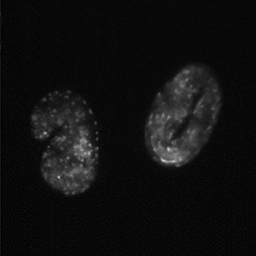
\includegraphics[width=0.23\columnwidth]{mypreprocess/3r.jpg}
		\label{fig:3r}
	}
	\subfigure
	{
		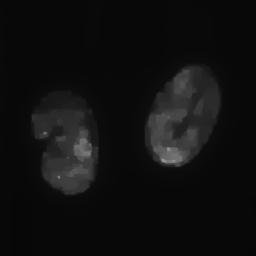
\includegraphics[width=0.23\columnwidth]{mypreprocess/3rtv.jpg}
		\label{fig:3rtv}
	}
	\subfigure
	{
		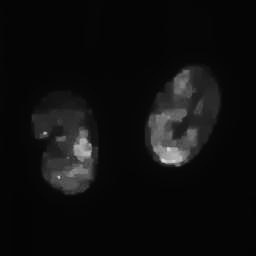
\includegraphics[width=0.23\columnwidth]{mypreprocess/3rtv_remapped.jpg}
		\label{fig:3rremap}
	}

	\subfigure	
	{
		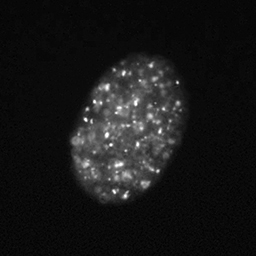
\includegraphics[width=0.23\columnwidth]{mypreprocess/4r.jpg}
		\label{fig:4r}
	}
	\subfigure
	{
		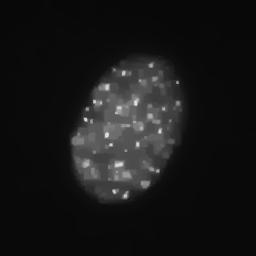
\includegraphics[width=0.23\columnwidth]{mypreprocess/4rtv.jpg}
		\label{fig:4rtv}
	}
	\subfigure
	{
		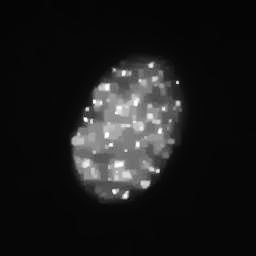
\includegraphics[width=0.23\columnwidth]{mypreprocess/4rtv_remapped.jpg}
		\label{fig:4rremap}
	}

	\subfigure	
	{
		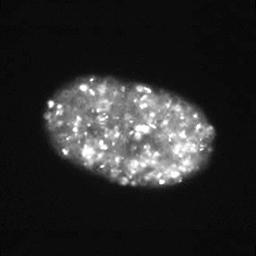
\includegraphics[width=0.23\columnwidth]{mypreprocess/5r.jpg}
		\label{fig:5r}
	}
	\subfigure
	{
		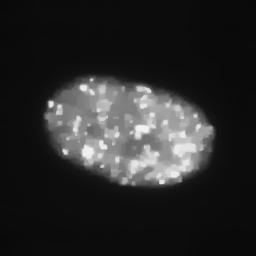
\includegraphics[width=0.23\columnwidth]{mypreprocess/5rtv.jpg}
		\label{fig:5rtv}
	}
	\subfigure
	{
		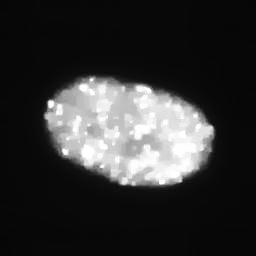
\includegraphics[width=0.23\columnwidth]{mypreprocess/5rtv_remapped.jpg}
		\label{fig:5rremap}
	}
	
	\caption{Original channel, TV denoised and remapped.}
	\label{fig:original_tv_remap}
\end{figure}

\begin{figure}[!h]
	\centering
	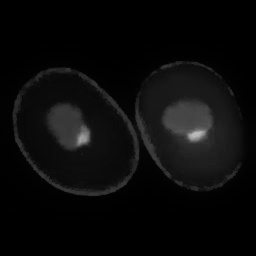
\includegraphics[width=0.5\columnwidth]{mypreprocess/1mixed.jpg}
	\caption{Mixed.}
	\label{fig:mixed}
\end{figure}

\begin{figure}[!h]
	\centering
	\subfigure[]
	{
		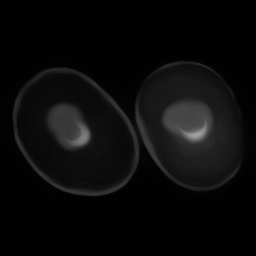
\includegraphics[width=0.23\columnwidth]{mypreprocess/1cedori.jpg}
		\label{fig:1mixed}
	}
	\subfigure[]
	{
		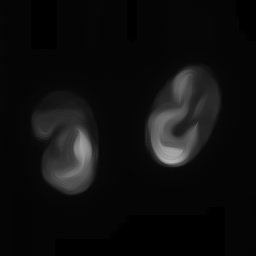
\includegraphics[width=0.23\columnwidth]{mypreprocess/3cedori.jpg}
		\label{fig:3mixed}
	}
	\subfigure[]
	{
		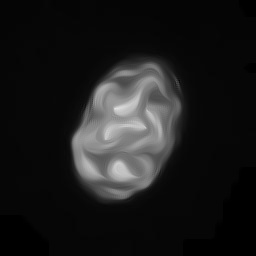
\includegraphics[width=0.23\columnwidth]{mypreprocess/4cedori.jpg}
		\label{fig:4mixed}
	}	
	\subfigure[]
	{
		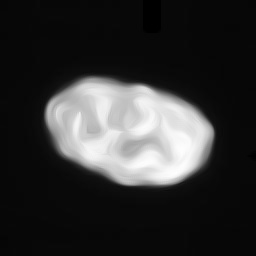
\includegraphics[width=0.23\columnwidth]{mypreprocess/5cedori.jpg}
		\label{fig:5mixed}
	}
	\caption{Final proxy after CED-ORI Filtering.}
	\label{fig:cedori}
\end{figure}

\begin{definition}[Parameter Settings]
	The results of the segmentations are presented in \Cref{tab:class_stats}. We compare four pre-processing schemes. In the table, the first scheme is denoted A and represents the results when using the raw gray level image; the  second scheme denoted B represents the results of using the coherence enhancing diffusion filter with optimised rotational invariance (CED-ORI) \citep{Weickert2002}, as done in \citep{Maska2013} and \citep{Kroon2009}. The parameters used are:
	$\sigma = 3.0, \, \rho = 5.0, \, c_1 = 1 \times 10^{-3}, \, c_2 = 1, \, \Delta t = 0.0015, \, n=20$.
	The third scheme, denoted  C in the table, is the results of having each image denoised using the following parameters: $\lambda = 1, \, \mu = 20,  \, \epsilon = 1 \times 10^{-3}$.
	The fourth scheme, denoted D in the table, is using the proposed scheme. The parameters for the TV denoising and CED-ORI are the same as previously presented. The additional parameters for the third step were set to: $\kappa_1 = 0.17, \, R_1 = 50, \, \kappa_2 = 0.55, \, R_2 = 225$. For the channel mixing step the weights used are shown in \Cref{tab:channel_weights}.
	
	A numerical comparison of each segmentation, in \Cref{tab:class_stats}, shows an increase in the general accuracy of the classification and the segmentation contours are smoother and fit the cell more appropriately.
	
	\begin{figure}[!h]
		\centering
		
		\subfigure[]
		{
			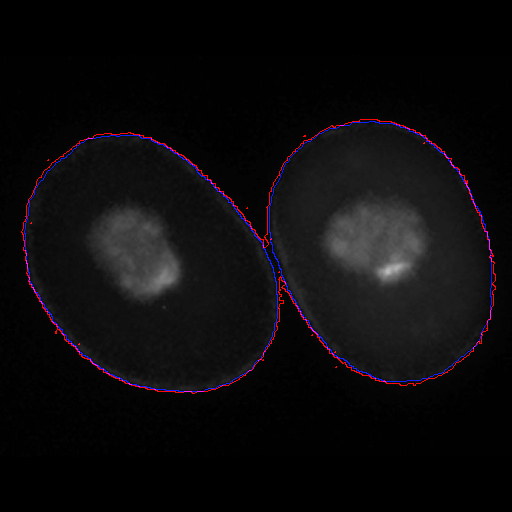
\includegraphics[width=0.23\columnwidth]{mypreprocess/1segno}
			\label{fig:1segno}
		}
		\subfigure[]
		{
			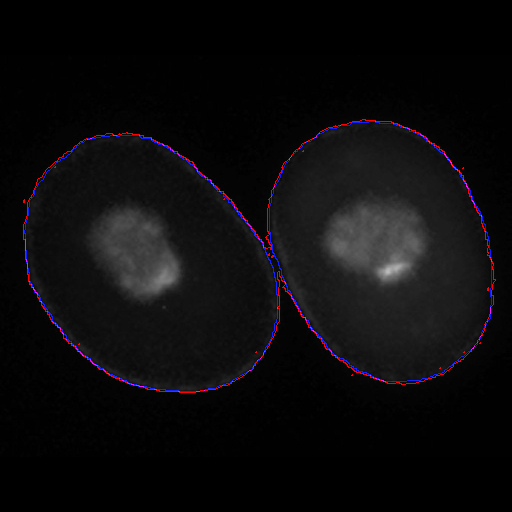
\includegraphics[width=0.23\columnwidth]{mypreprocess/1segced}
			\label{fig:1segced}
		}
		\subfigure[]
		{
			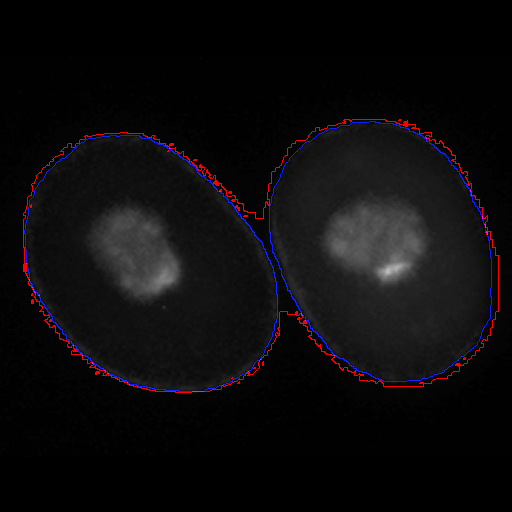
\includegraphics[width=0.23\columnwidth]{mypreprocess/1segtv}
			\label{fig:1segtv}
		}
		\subfigure[]
		{
			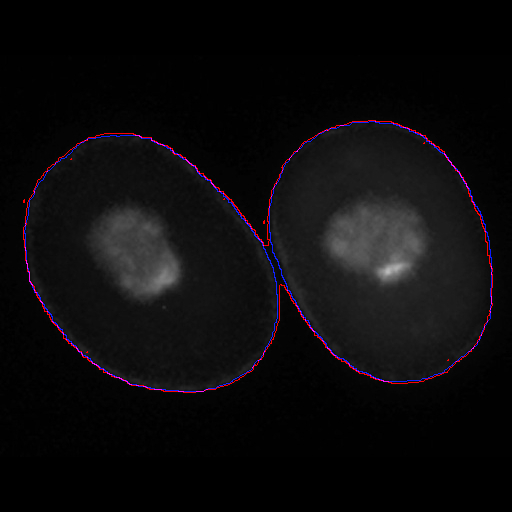
\includegraphics[width=0.23\columnwidth]{mypreprocess/1segscheme}
			\label{fig:1segscheme}
		}
		
		\subfigure[]
		{
			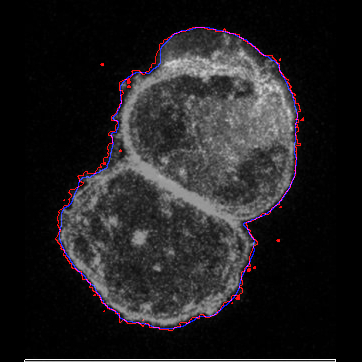
\includegraphics[width=0.23\columnwidth]{mypreprocess/2segno}
			\label{fig:2segno}
		}
		\subfigure[]
		{
			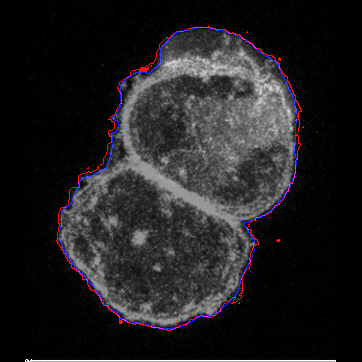
\includegraphics[width=0.23\columnwidth]{mypreprocess/2segced}
			\label{fig:2segced}
		}
		\subfigure[]
		{
			\includegraphics[width=0.23\columnwidth]{mypreprocess/2segtv}
			\label{fig:2segtv}
		}
		\subfigure[]
		{
			\includegraphics[width=0.23\columnwidth]{mypreprocess/2segscheme}
			\label{fig:2segscheme}
		}
		
		\subfigure[]
		{
			\includegraphics[width=0.23\columnwidth]{mypreprocess/3segno}
			\label{fig:3segno}
		}
		\subfigure[]
		{
			\includegraphics[width=0.23\columnwidth]{mypreprocess/3segced}
			\label{fig:3segced}
		}
		\subfigure[]
		{
			\includegraphics[width=0.23\columnwidth]{mypreprocess/3segtv}
			\label{fig:3segtv}
		}
		\subfigure[]
		{
			\includegraphics[width=0.23\columnwidth]{mypreprocess/3segscheme}
			\label{fig:3segscheme}
		}
		
		\subfigure[]
		{
			\includegraphics[width=0.23\columnwidth]{mypreprocess/4segno}
			\label{fig:4segno}
		}
		\subfigure[]
		{
			\includegraphics[width=0.23\columnwidth]{mypreprocess/4segced}
			\label{fig:4segced}
		}
		\subfigure[]
		{
			\includegraphics[width=0.23\columnwidth]{mypreprocess/4segtv}
			\label{fig:4segtv}
		}
		\subfigure[]
		{
			\includegraphics[width=0.23\columnwidth]{mypreprocess/4segscheme}
			\label{fig:4segscheme}
		}
		
		\subfigure[]
		{
			\includegraphics[width=0.23\columnwidth]{mypreprocess/5segno}
			\label{fig:5segno}
		}
		\subfigure[]
		{
			\includegraphics[width=0.23\columnwidth]{mypreprocess/5segced}
			\label{fig:5segced}
		}
		\subfigure[]
		{
			\includegraphics[width=0.23\columnwidth]{mypreprocess/5segtv}
			\label{fig:5segtv}
		}
		\subfigure[]
		{
			\includegraphics[width=0.23\columnwidth]{mypreprocess/5segscheme}
			\label{fig:5segscheme}
		}
		
		\caption{Segmentation results.}
		\label{fig:schemesegmentationresults}
	\end{figure}
	
	\begin{table}[!h]
		\renewcommand{\arraystretch}{1.3}
		\caption{Classification Statistics[A - Original gray scale image, B - CED-ORI only, C - Anisotropic TV denoising only, D - Proposed Preprocessing Scheme]}
		\label{tab:class_stats}
		\centering
		\begin{tabular}{|c|c|c|c|c|}
			\hline
			&   & Sensitivity & Specificity & F1 score\\ \hline
			Image 1  	& A & 0.956157 & 0.974129 & 0.975526 \\
			& B & 0.952542 & 0.971822 & 0.974790 \\
			& C & 0.778485 & 0.839000 & 0.874881 \\
			& D & 0.981447 & 0.989360 & 0.987344 \\ \hline
			
			Image 2     	& A & 0.967517 & 0.981730 & 0.979699 \\
			& B & 0.972583 & 0.984701 & 0.980968 \\
			& C & 0.932064 & 0.960116 & 0.963754 \\
			& D & 0.973092 & 0.985008 & 0.980745 \\ \hline
			
			Image 3     	& A & 0.977581 & 0.997342 & 0.704079 \\
			& B & 0.967342 & 0.993423 & 0.945607 \\
			& C & 0.980888 & 0.996411 & 0.924565 \\
			& D & 0.973788 & 0.994494 & 0.972452 \\ \hline
			
			Image 4     	& A & 0.984491 & 0.961890 & 0.964425 \\
			& B & 0.998658 & 0.999674 & 0.972736 \\
			& C & 0.878951 & 0.964813 & 0.934818 \\
			& D & 0.999495 & 0.999873 & 0.989058 \\ \hline
			
			Image 5    	& A & 0.999931 & 0.999980 & 0.966254 \\
			& B & 0.997783 & 0.999318 & 0.988121 \\
			& C & 0.982536 & 0.994460 & 0.988247 \\
			& D & 1.000000 & 1.000000 & 0.977193 \\ \hline
		\end{tabular}
	\end{table}
	
	\begin{table}[!h]
		\renewcommand{\arraystretch}{1.3}
		\caption{Channel Mixing Weights}
		\label{tab:channel_weights}
		\centering
		\begin{tabular}{|c|c|c|c|}
			\hline
			& $w_R$	& $w_G$	& $w_B$\\ \hline
			Image 1 	& 0.2 	& 0.6 	& 0.2 \\ \hline
			Image 2    	& 0.5 	& 0.5 	& 0.0 \\ \hline
			Image 3		& 1.0 	& 0.0 	& 0.0 \\ \hline
			Image 4		& 1.0 	& 0.0 	& 0.0 \\ \hline
			Image 5		& 1.0 	& 0.0 	& 0.0 \\ \hline
		\end{tabular}
	\end{table}
\end{definition}

\begin{definition}[Execution Time]
	The scheme was implemented in C++ using OpenCV 2.3.4. There were no run-time optimisations performed in the code nor any complexity reduction of algorithms. The Operating System used was Ubuntu 13.10 on a Core 2 Duo 1.3GHz with this 2GB RAM. To get the results, the running times to process 744 images  were analysed. The results are shown in \Cref{tab:results_runningtime}. The mean running time versus the image size can be seen in \Cref{fig:results_runningtime}. As can be seen from \Cref{tab:results_runningtime}, the bulk of the processing time is spent on denoising and intra-region smoothing.
	
	\begin{table}[!h]
		\renewcommand{\arraystretch}{1.3}
		\caption{Running Time Results}
		\label{tab:results_runningtime}
		\centering
		\begin{tabular}{|c|c|c|c|c|c|}
			%& & \multicolumn{3}{c}{} \\ \hline
			\hline
			Chn		& Dims 		& Mean	& St. Dev	& \%TV	& \%CEDORI \\ \hline
			1 			& $64\times64$	& $4.63$	& $1.02$	& $24.58$& $74.50$\\
			& $128\times128$	& $14.44$& $4.02$& $19.12$& $80.61$ \\
			& $192\times192$	& $31.73$& $8.56$& $22.42$& $77.44$ \\
			& $256\times256$	& $58.12$& $14.40$& $22.58$& $77.36$ \\
			& $320\times320$	& $97.72$& $24.91$& $19.86$& $80.09$ \\
			& $384\times382$	& $147.96$& $37.94$& $18.06$& $81.91$ \\
			& $448\times448$	& $188.19$& $41.16$& $18.81$& $81.17$ \\
			& $512\times512$	& $250.24$& $52.16$& $17.68$& $82.30$ \\
			\hline
			\multicolumn{4}{|r}{Mean} & $20.39$ & $79.42$ \\
			\multicolumn{4}{|r}{St. Dev} & $2.50$ & $2.72$ \\
			\hline
			
			%          	\hline
			2 		 	& $64\times64$	&$5.77$	 &$1.94$	 &$39.45$& $59.78$ \\
			& $128\times128$	&$17.20$	 &$6.86$ &$32.11$& $67.68$ \\
			& $192\times6192$&$38.84$	 &$16.02$&$36.63$& $63.27$ \\          			
			& $256\times256$	&$71.24$	 &$26.47$&$36.84$& $63.11$ \\
			& $320\times320$ &$117.12$&$42.02$&$33.14$	& $66.83$ \\
			& $384\times384$ &$174.68$&$60.64$&$30.59$	& $69.83$ \\
			& $448\times448$ &$223.59$&$69.34$&$31.66$	& $68.32$ \\
			& $512\times512$ &$294.50$&$86.74$&$30.05$	& $69.93$ \\
			\hline
			\multicolumn{4}{|r}{Mean} & $33.81$ & $66.04$ \\
			\multicolumn{4}{|r}{St. Dev} & $3.41$ & $3.59$ \\
			\hline
			
			%            	\hline
			3 		  	& $64\times64$ 	&$6.91$ &$2.85$ & $49.42$	&$49.92$ \\
			& $128\times128$ &$19.96$ &$9.69$ &$41.50$	&$58.32$ \\
			& $192\times192$ &$45.96$ &$23.49$ &$46.44$&$53.47$ \\
			& $256\times256$	&$84.37$ &$38.54$ &$46.66$&$53.29$ \\
			& $320\times320$ &$136.53$&$59.14$ &$42.64$&$57.33$ \\
			& $384\times382$ &$201.40$&$83.34$ &$39.80$&$60.18$ \\
			& $448\times448$ &$258.98$&$97.52$ &$41.00$&$58.98$ \\
			& $512\times512$ &$338.75$&$121.32$&$39.19$&$60.80$ \\
			\hline
			\multicolumn{4}{|r}{Mean} & $43.33$ & $56.54$ \\
			\multicolumn{4}{|r}{St. Dev} & $3.72$ & $3.87$ \\
			\hline
		\end{tabular}
	\end{table}
	
	\begin{figure}[!h]
		\centering
		\includegraphics[width=0.80\columnwidth]{mypreprocess/runningtime}
		\caption{Running time vs Image size}
		\label{fig:results_runningtime}
	\end{figure}
\end{definition}
%----------------------------------------------------------------------------------------
%	SECTION 4
%----------------------------------------------------------------------------------------

\section{Discussion}
\label{sec:preprocessschemediscussion}

We have  presented a scheme that adjusts the properties of an image such that more accurate segmentation can be obtained. Experiments  performed on 2D fluorescence microscopy image data show that the proposed scheme outperforms the existing techniques. One  limitation of the scheme  is the tuning of the various parameters. The running time can also be reduced by  using parallel computing or by optimizing algorithms used.
